\section{Portation implementation}
%todo introduction to section
\subsection{Gradle scripts}


\section{Application implementation}
%todo introduction to section

\subsection{Application structure} % describe inner structure not ui
Application consists from three screens. First screen is displayed after start of the application and it is used for
settings of calculation time limit and algorithm. These parameters are packed in bundle and passed to next screen after
user clicks on the Open file button placed on this screen. Second screen consist of list of example vrp files which is
provided by RecyclerView component. User selects one of the files and its name is passed to last screen together with
parameters from the first one. According to name, vrp file is open on the last screen and after click on start button
asynchronous process for calculation is created. More details about individual components are described below.

\subsubsection{Activities and fragments}
Initialy, all the application screens was implemented as activities. However, it turns out that activities have problems
with data storing and after some change of configuration (for example rotation of screen or restoring application from
background) destroyes background process and totally recreates activity. Thus framgments were used instead.

Fragments represents part of an Activity. Activity can contain multiple fragments and they can be replaced with another
fragments. They can be presented as modular section of an activity with own lifecycle.

Figure \ref{activityFragment} shows usage of fragments and activities in this application. Only one activity is presented and it
contains action bar and place for fragments. Compared to activites, only part for fragment changes and if new screen is
required this part is replaced with another fragment. Activity is recreated only in case when application is restarted
or configuration is changed.

For proper storage of state in fragment \texttt{setRetainInstance(true);} has to be called in method \texttt{onCreate()}
of current fragment.

\begin{figure}[h!]
    \centering
    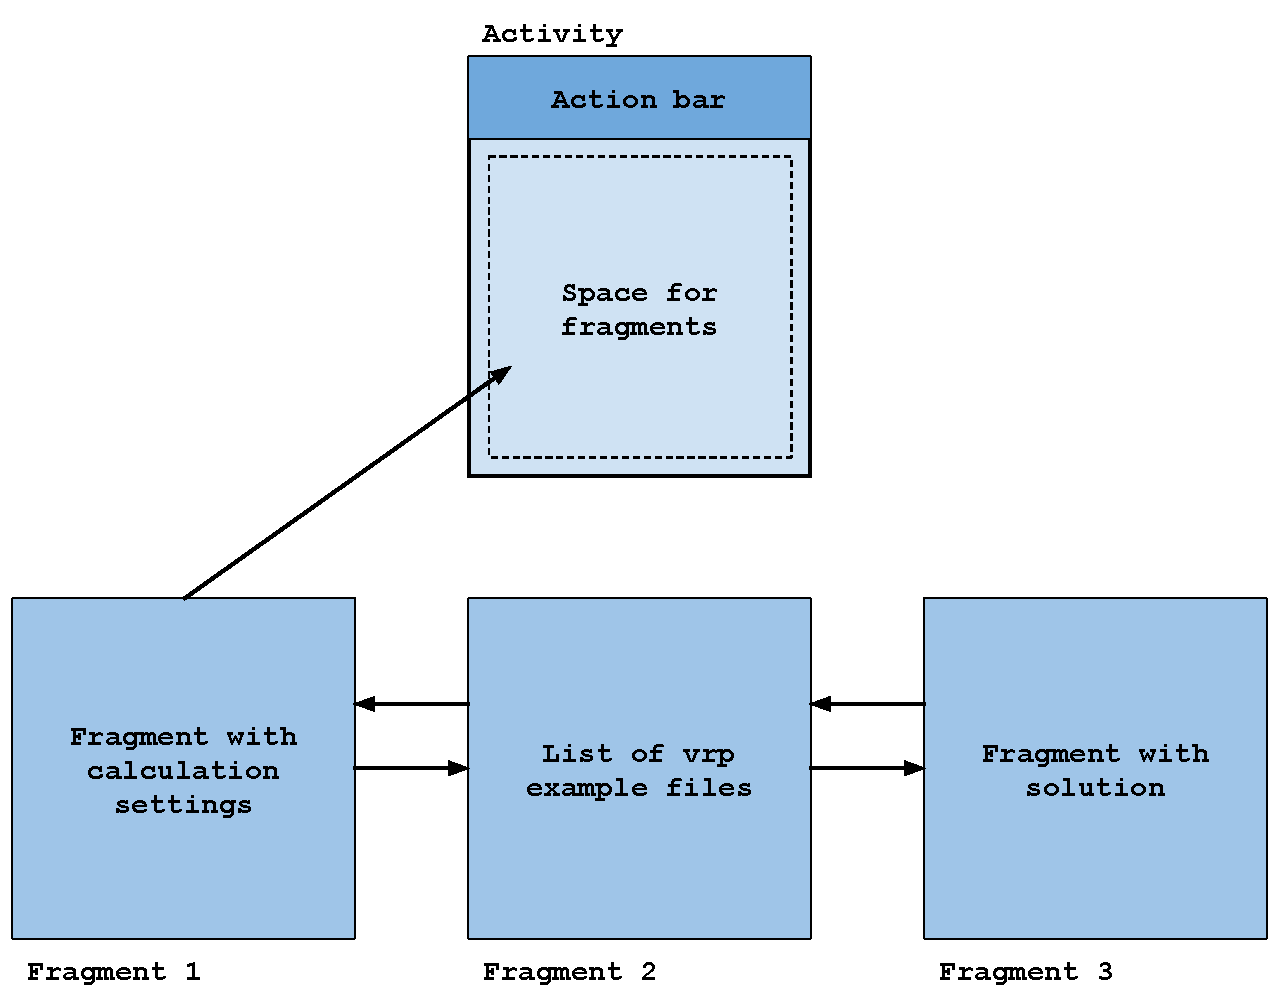
\includegraphics[scale=0.7]{fig/act_frag.pdf}
    \caption{Activity and fragments in application}
    \label{activityFragment}
\end{figure}

\subsubsection{Fragment components}
In following section, important component of application is described. Especially, these components are related to
background process and not graphical layout of application which is described in Section \ref{guiSection}.

\paragraph{List of files}
Second screen consist mainly from list of vrp example files. This list is implemented by \texttt{RecyclerView}
component. This component simplifies data displaying to list and provides basic patterns of behavior.

\paragraph{Solver asynchronous process}
After button for calculation start is pressed, asynchronous process is created. This process sets, build and run solver
with required parameters. Listener is added to solver to publish process every time when new best solution is found.
Asynchronous process is represented by \texttt{VrpSolverTask} class which extends \texttt{AsyncTask}. \texttt{AsyncTask}
class enables changes of gui, perform background operations and publishing results.

\paragraph{Solution painter}
When file is selected from list in second screen unsolved solution is painted. After start of caculation, every time
when new best solution is found solution painter draws it. Solution painter is represented by \texttt{VrpPainter} class
and it is partially modified \texttt{VehicleRoutingSolutionPainter} class from Optaplanner project. Because Android
does not support awt and swing graphic libraries, it was rewritten to use android tools. Also some other changes was
done like new appearance of customers, material design colors and more.

\subsection{Porting of Vehicle Routing Problem}
%todo introduction to subsection

\paragraph{Vehicle Routing Problem definition}
Without defining of the problem, application cannot work. Vehicle routing problem is defined by
\texttt{VehicleRoutingSolution} class which implements \texttt{Solution} interface. This class contains all information
about solved problem (list of all customers, depots and vehicles) and Solver use it together with solver configuration
to solve the problem. \texttt{Customer} class is marked as planned entity which contains \texttt{Standstill} planning
variable. More information about Vehicle Routing Problem definition can be found in OptaPlanner documentation
\cite{OptaPlannerDoc}.

\paragraph{Solver configurations}
In this application, it is possible to use three algorithms and set time limit of calculation. These configurations
including problem definition abd score calculator are stored in xml file from which is Solver built. For each algorithm
is created such file and it is selected according to the choice. Time limit is additionally set after Solver is created.

\paragraph{Score calculator}
Every solution has own score and this score must be calculated one of the three methods described in Section
\ref{scoreConfigSection}. For score calculation in this application, \texttt{VehicleRoutingEasyScoreCalculator} class
which implements \texttt{EasyScoreCalculator} is used. This class calculates hard and soft score of solution. Hard score
is computed as load of cars above their capacity. Soft score is calculated as total distance of cars. In case of time
window variant, delay against due time of arrival is added to hard score.

\paragraph{Vrp example files}
Example .vrp files are used for problem datasets. These files are taken from Vehicle Routing problem part of original
Optaplanner application. They cointains informations about number and capacity of vehicles, position and demand of
customers and position of depot. This application includes 36 example files in total.

\paragraph{Vehicle routing importer}
Example files are stored in specific vrp text format and have to be transformed into Vehicle routing solution. For this
purpose, \texttt{VehicleRoutingImporter} class is imported and used from original Optaplanner application.

\section{Graphical user interface}\label{guiSection}
%todo introduction to section

\subsection{Application screens}
Every application consists of fragments or activities which are collectively called screens. Using controls, it is
possible to move from one screen to another or change its appearance or behavior. This application is composed from
three screens. These screens can be seen in Figure \ref{screens}. The third screen is displayed with unsolved and with
solved solution.

\paragraph{Main screen}
Main screen is displayed after the application is started. It consists from action bar, welcome text, setting elements
and button to continue to another screen. Action bar contains application name and buttons for displaying legend and
application informations dialogs. Welcome text provides some basic instruction for the user. Two controls are present
for calculation options of the problem. It is possible to set time limit in seconds using Number picker and Spinner
allows select one of the three supported algorithms. Last element on this screen is Open file button which opens screen
with list of vrp files.

\paragraph{Screen with vrp files list} After Open file button from main screen is pressed this screen is displayed. It
also contains action bar but it is very litimed because no controls are required there. Basically, whole screen is
filled with list of vrp files. These example files were used from OptaPlanner project \cite{OptaPlannerPages}. After
pressing the selected file it is switched to last screen which displays problem and its solution.

\paragraph{Screen of solution}
This screen is used to displaying unsolved and solved solution. It contains action bar with all items as shown in Figure
\ref{actionBar}. Compared to the main screen, action bar has additionally button for displaying Navigation drawer and
button for start and end of the solution process. On the bottom of the screen, Progress bar is placed. This component
is used for displaying approximate remaining time. Rest of screen is filled with component which draws current solution.
This component draws unsolved solution at the beginning and after start button is pressed it draws best solution after
solver finds some. Individual elements represents:

\begin{itemize}
  \item \textbf{Circle with a number} -- customer with his demand
  \item \textbf{Building image} -- depot from which depart vehicles
  \item \textbf{Car image} -- vehicle with its color
  \item \textbf{Solid line} -- vehicle road to customer
  \item \textbf{Dashed line} -- vehicle road to depot
  \item \textbf{Sector on a circle} -- time windows for vehicle arrival
  \item \textbf{Line on a circle} -- vehicle arrival time
\end{itemize}


\begin{figure}[h!]
    \centering
    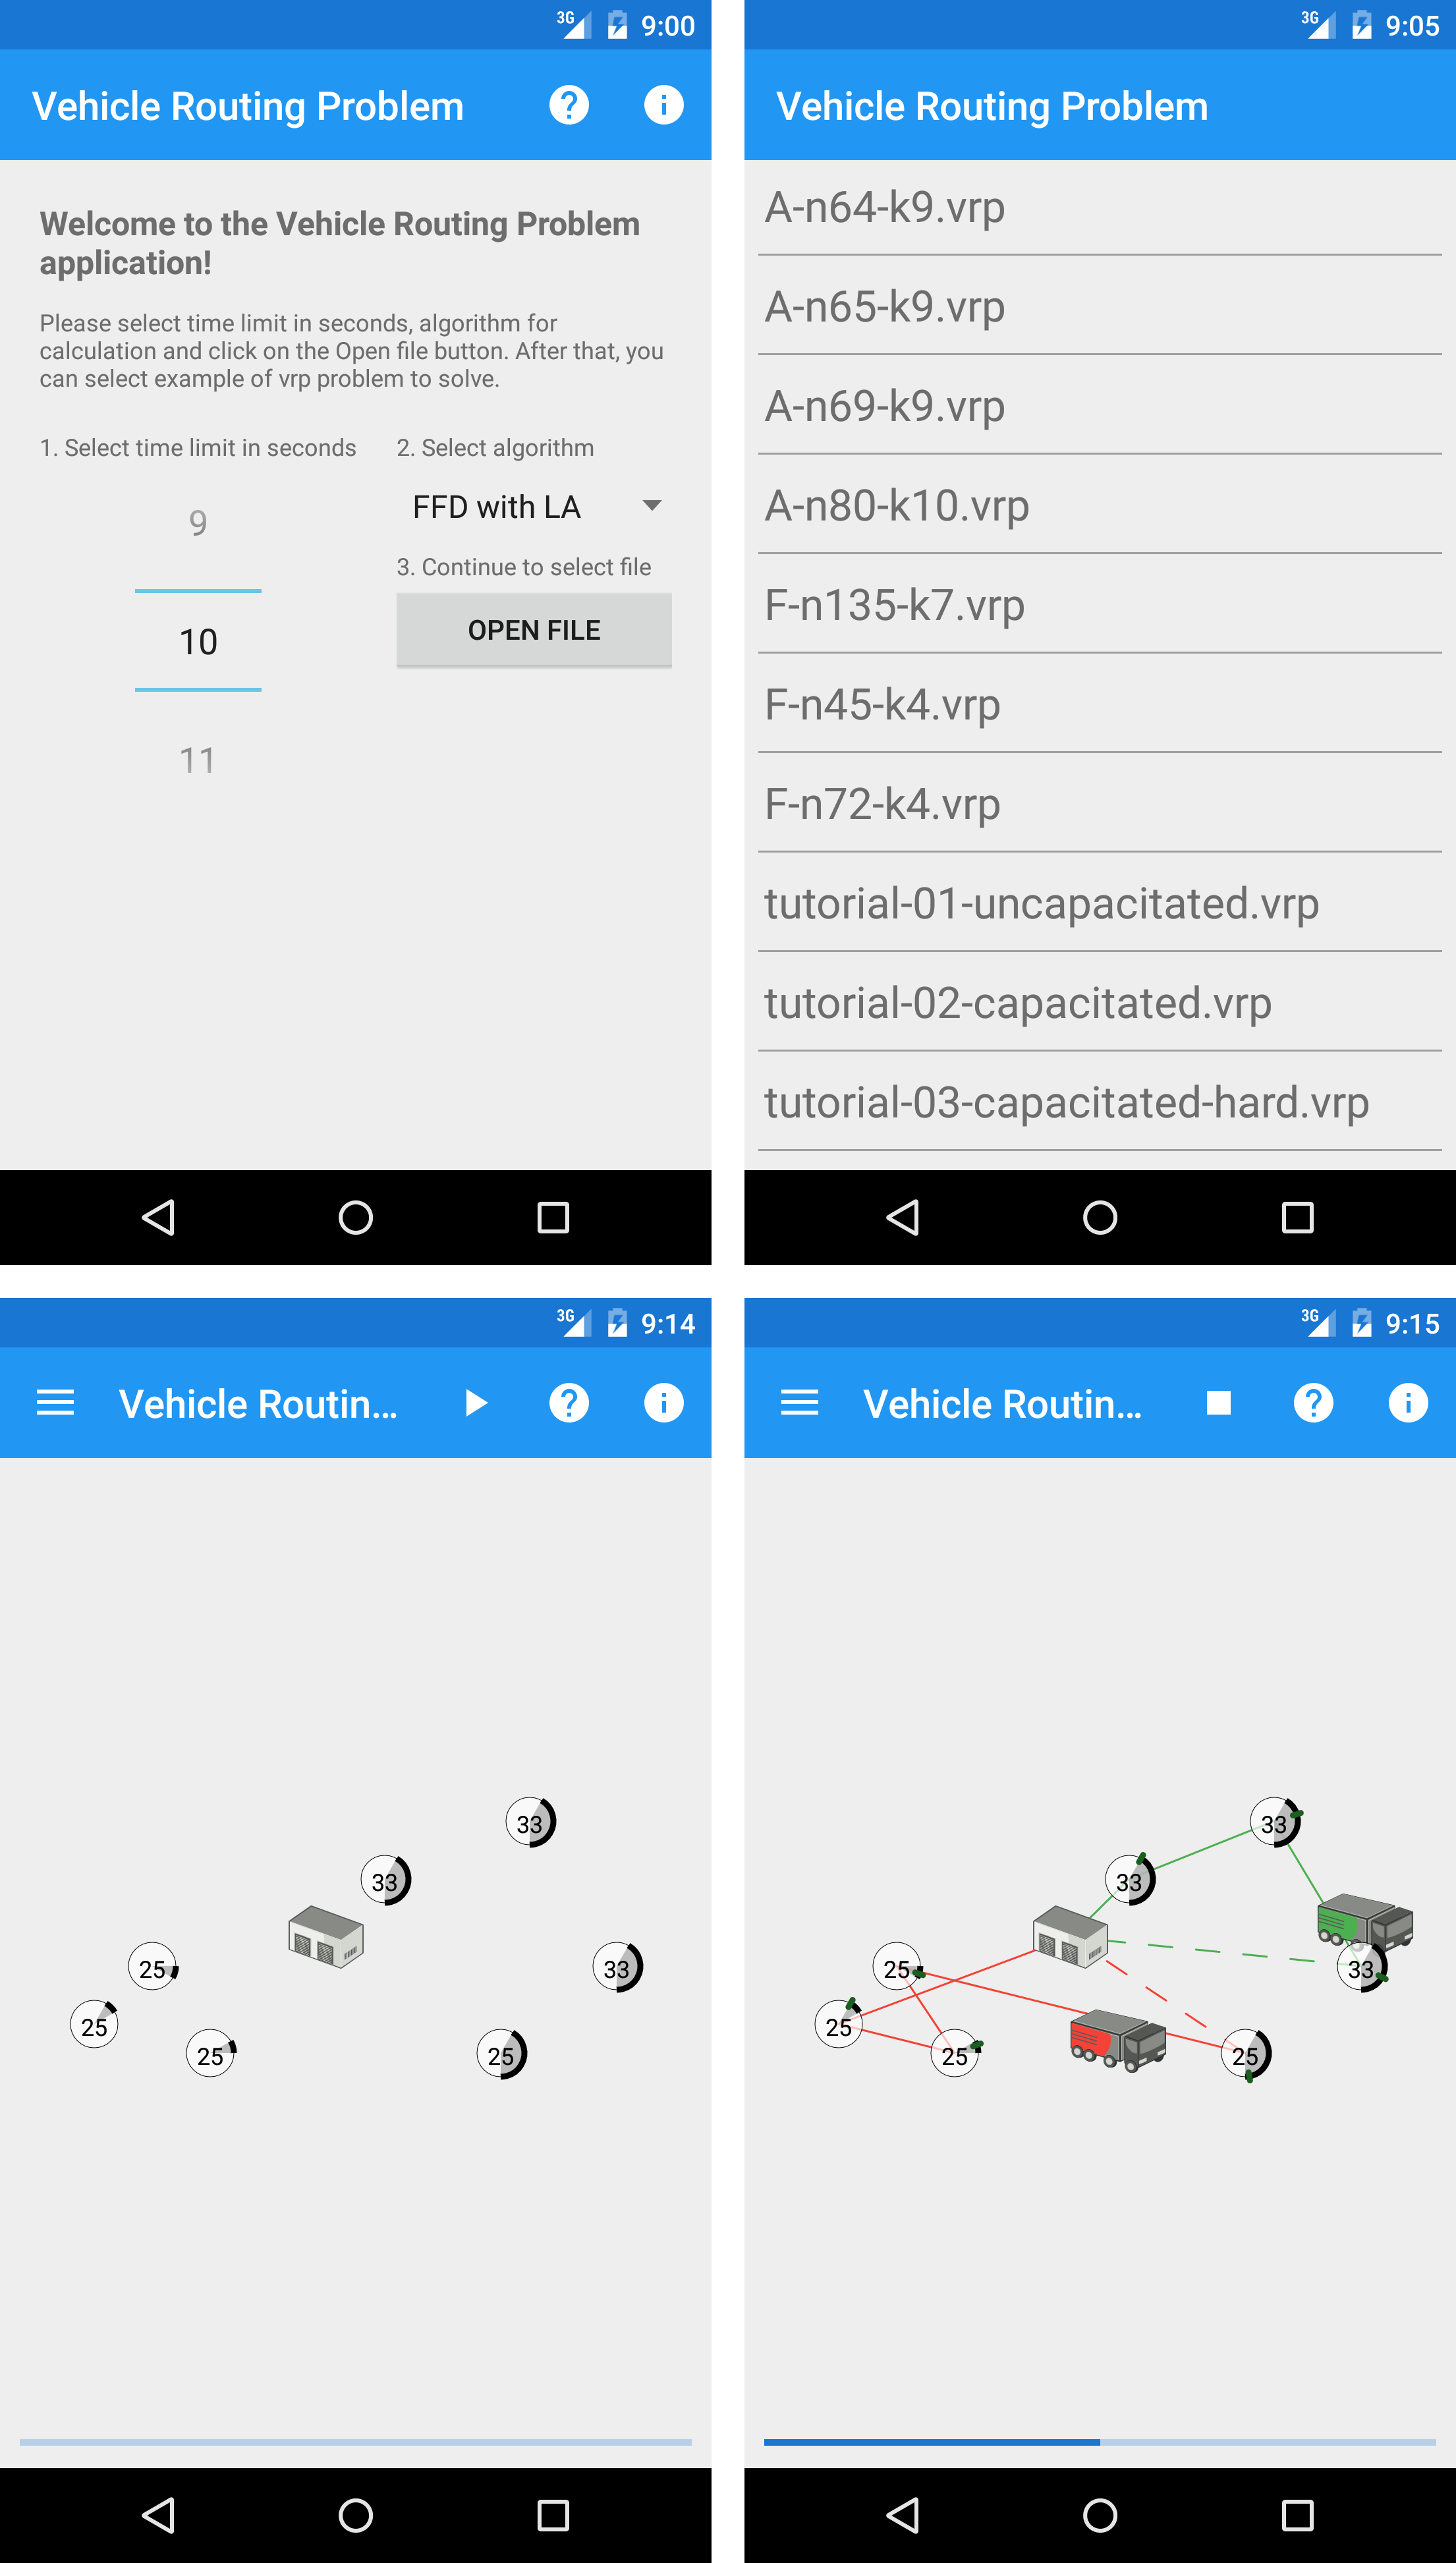
\includegraphics[scale=0.15]{fig/screens.png}
    \caption{Application screens -- main screen, list of vrp files, screen with unsolved and solved solution}
    \label{screens}
\end{figure}

\subsection{Application components}
%todo introduction to subsection

\subsubsection{Action bar}
Action bar is a panel on top of the screen that provides basic user action and informations about user navigation. It
always contains application name, optionally actions buttons for quick invocation of application functionalit and
overflow button on the right side for diplaying other applications options.

Action bar is diplayed on every screen of this application but it changes depending on required functions on actual
screen. Figure \ref{actionBar} show action bar of screen where solved problems are shown. The panel contains buttons for
displaying of navigation drawer and dialogs which are described below and application name.

\begin{figure}[h!]
    \centering
    
\includegraphics[scale=0.15]{fig/action_bar.png}
    \caption{Action bar}
    \label{actionBar}
\end{figure}

\subsubsection{Navigation drawer}
Navigation drawer is a panel that displays application navigation on the left edge of the screen. By default, it is
hidden and it could be displayed by touch the left icon on the action bar. Also it could be displayed whe a user swipes
with a finger from the left edge of the screen to the right. Opposite procedure makes navigation drawer invisible.

This application uses navigation drawer for displaying important computing data. Figure \ref{navigationDrawer} displays
visible panel on the left side of the application. First item shows hard and soft score of currently the best solution
found. Second item holds total distance of all cars. Other items are linked to cars of the problem. Every car has own
parameters -- color, name and capacity. These three are static and do not change during the calculation. Last parametr
is actual load of the vehicle.

\begin{figure}[h!]
    \centering
    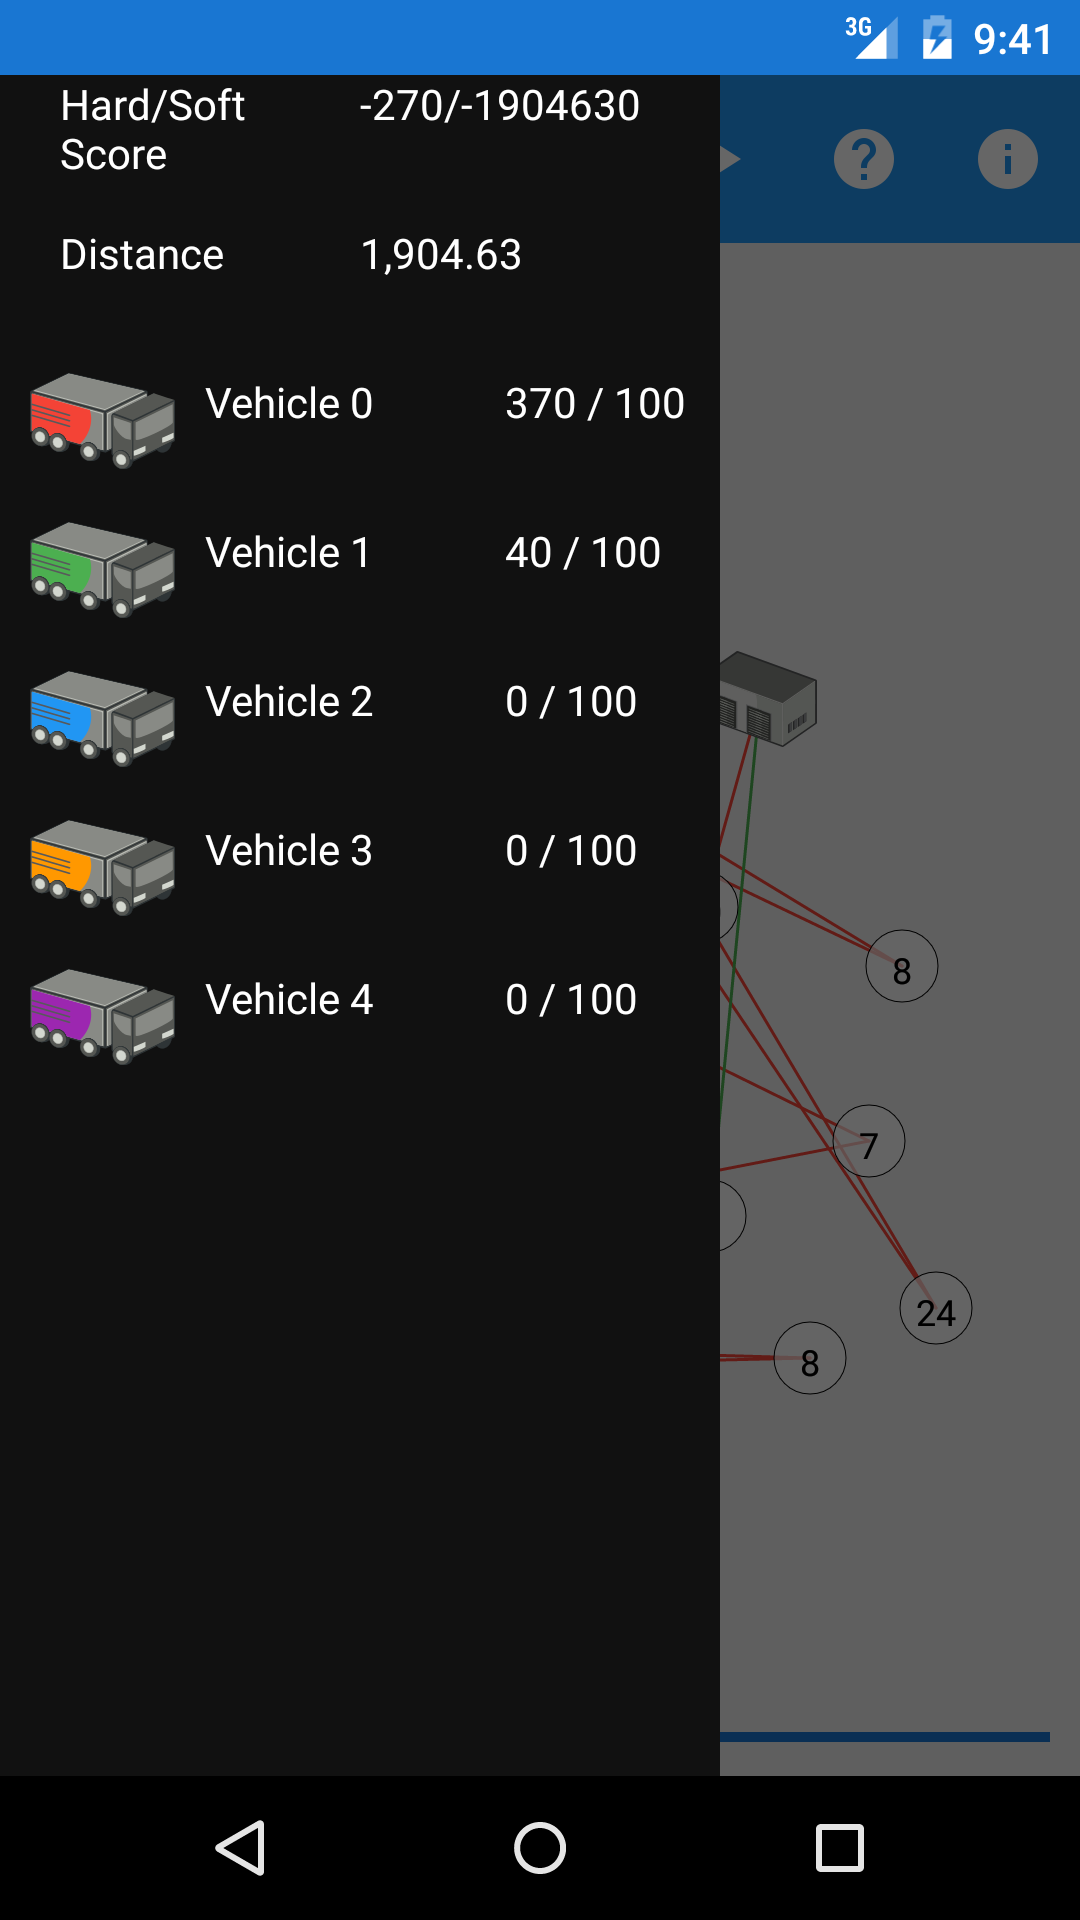
\includegraphics[scale=0.15]{fig/nav_drawer.png}
    \caption{Navigation drawer with actual data}
    \label{navigationDrawer}
\end{figure}

\subsubsection{Dialogs}
Dialogs are small windows which displays some significant informations or are used for user interaction with a decision
that decides on further actions. Dialogs are always located above all other parts of the application

Figure \ref{dialogs} shows all three dialogs which are used in the application. Two of them can be retrieved directly from the
action bar by clicking on the icon with a question mark or the informative icon. First dialog contains application
legend for understanding what is displayed on the screen and second dialog briefly describes the application. Third
dialog is displayed only solving is running and user clicks on the back button. Dialog asks the user if he wants to end
the ongoing calculation.

\begin{figure}[h!]
    \centering
    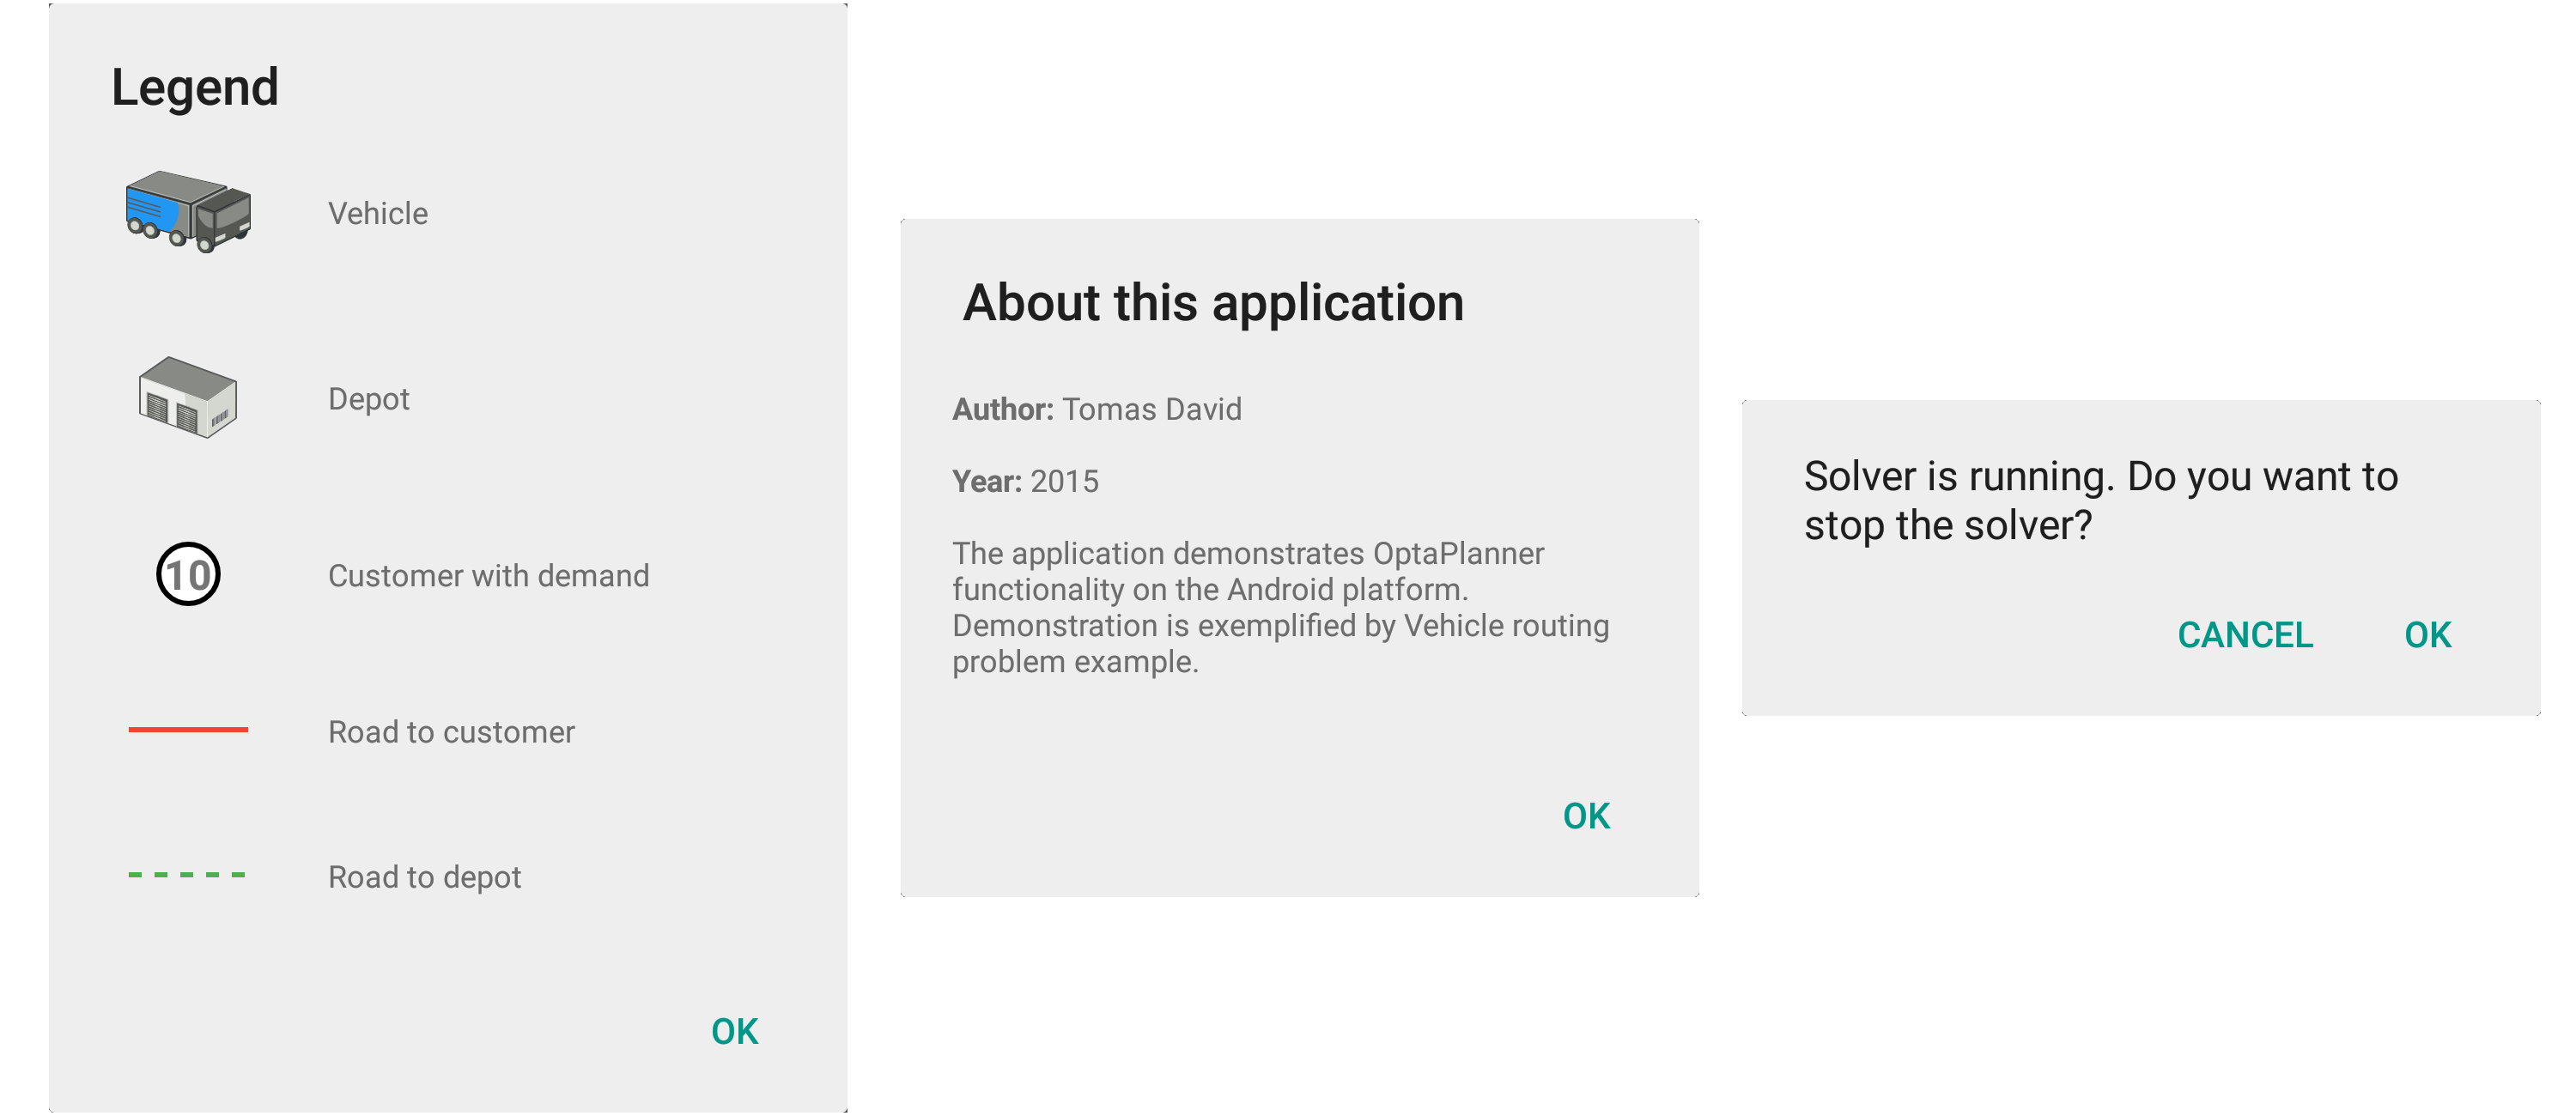
\includegraphics[scale=0.15]{fig/dialogs.png}
    \caption{dialogs used in the application}
    \label{dialogs}
\end{figure}
